\section{Average False Positive Error}\label{section:averageError}

Apart from the number of false positive and false negative evaluations, the distances of the false positives between the wrongly estimated scenes is another critical performance metric. If the false positive is close to the threshold and the distance is relatively small, then the result won't be influenced much. However, if the distance between wrongly matched scenes is very large, the negative impact on the result will be significant.\par
This section analyzes distances for every false positive result during the simulation in every environment. The exact distances for every false positive evaluation for both approaches are shown in Figures \ref{fig:averageFPErrorWarehouse}, \ref{fig:averageFPErrorHouse}, and \ref{fig:averageFPErrorHospital}. The average and maximal error distance for each approach in each environment, together with the comparison with the visual place recognition used in the OpenRatSLAM, is shown in the table \ref{tab:averageFPError}.\par

\begin{figure}[!tbp]
    \centering
    \subfloat[1st stage only]{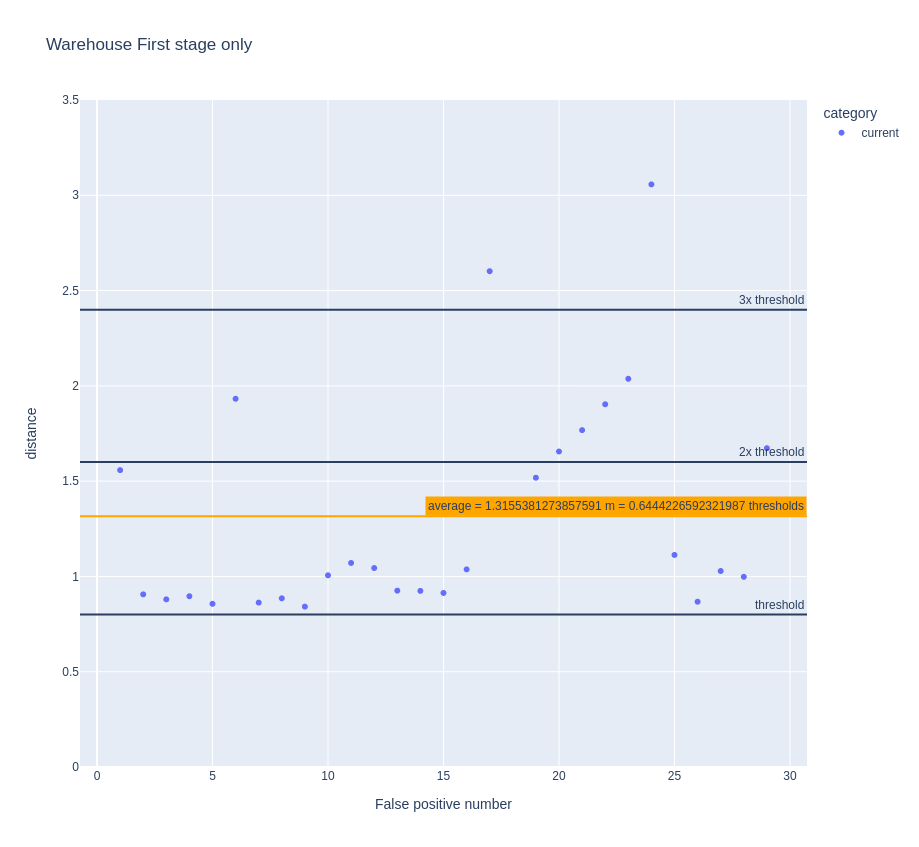
\includegraphics[width=0.5\textwidth]{warehouseFirstStageFalsePositiveDistances.png}\label{fig:FPErr11}}
    \hfill
    \subfloat[Both stages]{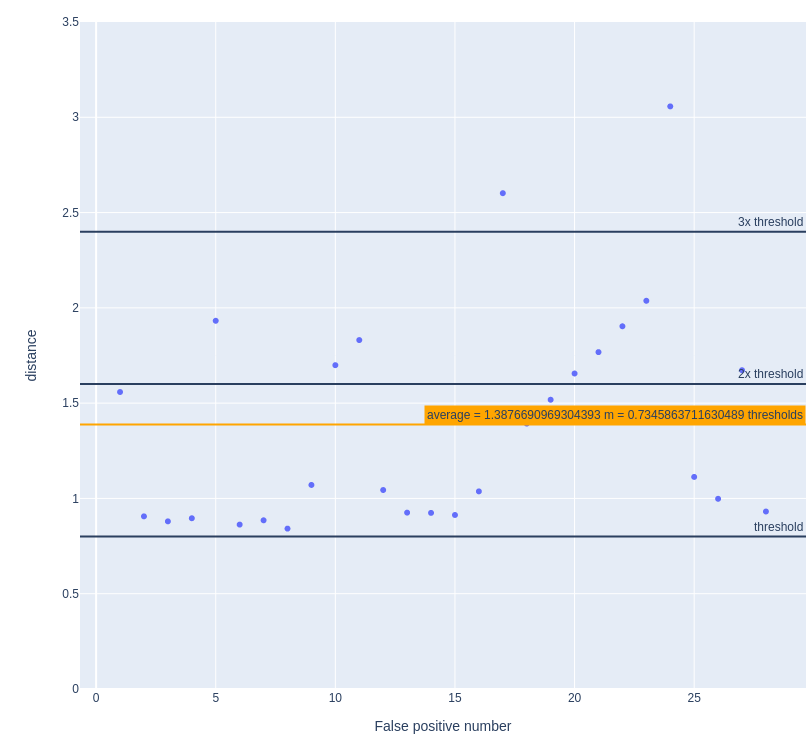
\includegraphics[width=0.5\textwidth]{warehouseBothStagesFalsePositiveDistances.png}\label{fig:FPErr12}}
    \caption{False positive distances in the warehouse environment}
    \label{fig:averageFPErrorWarehouse}
\end{figure}

\begin{figure}[!tbp]
    \centering
    \subfloat[1st stage only]{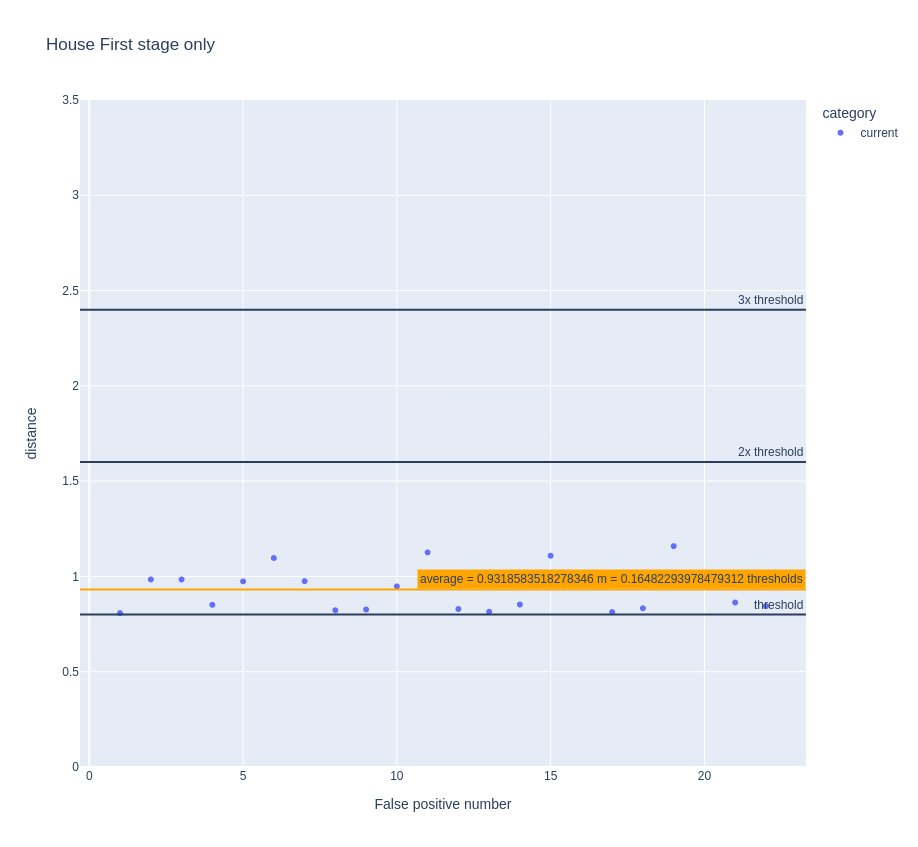
\includegraphics[width=0.5\textwidth]{houseFirstStageFalsePositiveDistances.png}\label{fig:FPErr21}}
    \hfill
    \subfloat[Both stages]{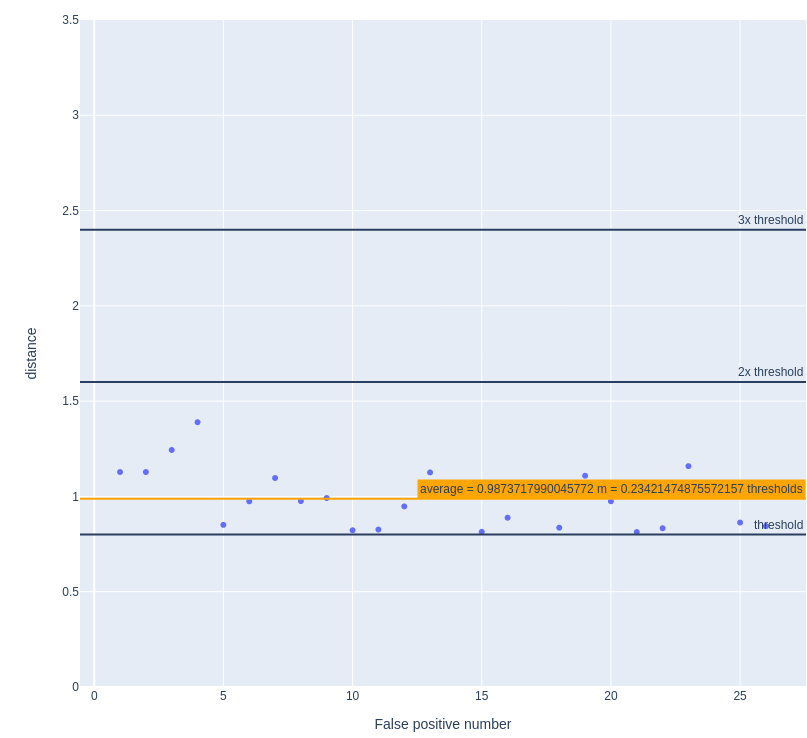
\includegraphics[width=0.5\textwidth]{houseBothStagesFalsePositiveDistances.png}\label{fig:FPErr22}}
    \caption{False positive distances in the house environment}
    \label{fig:averageFPErrorHouse}
\end{figure}

\begin{figure}[!tbp]
    \centering
    \subfloat[1st stage only]{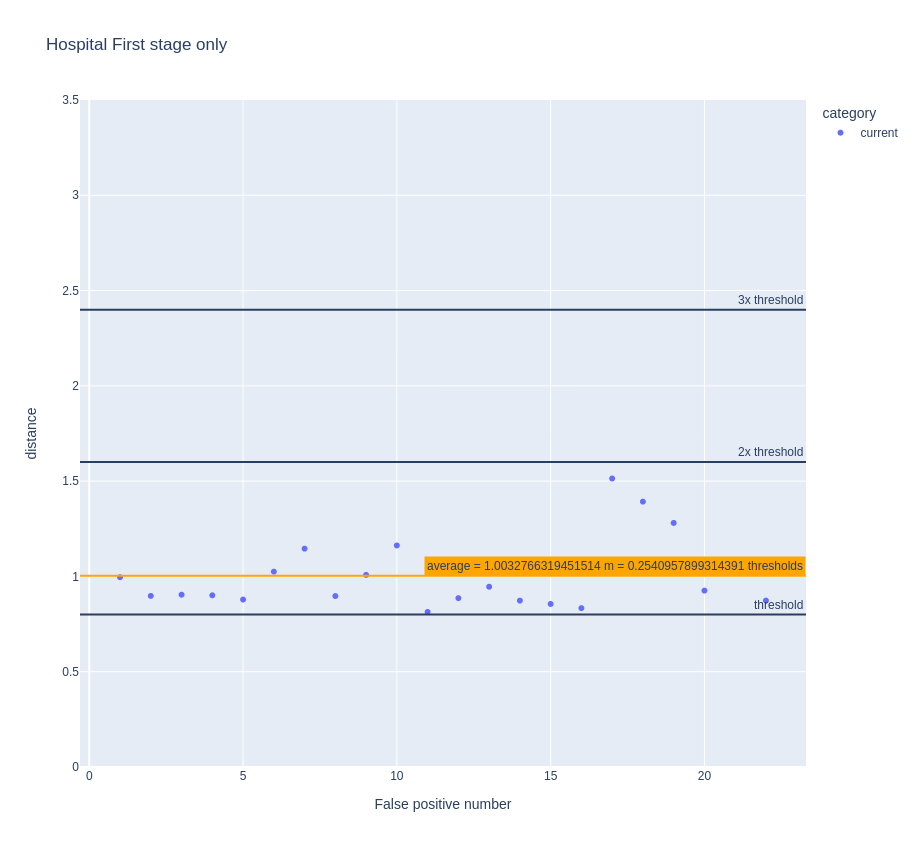
\includegraphics[width=0.5\textwidth]{hospitalFirstStageFalsePositiveDistances.png}\label{fig:FPErr31}}
    \hfill
    \subfloat[Both stages]{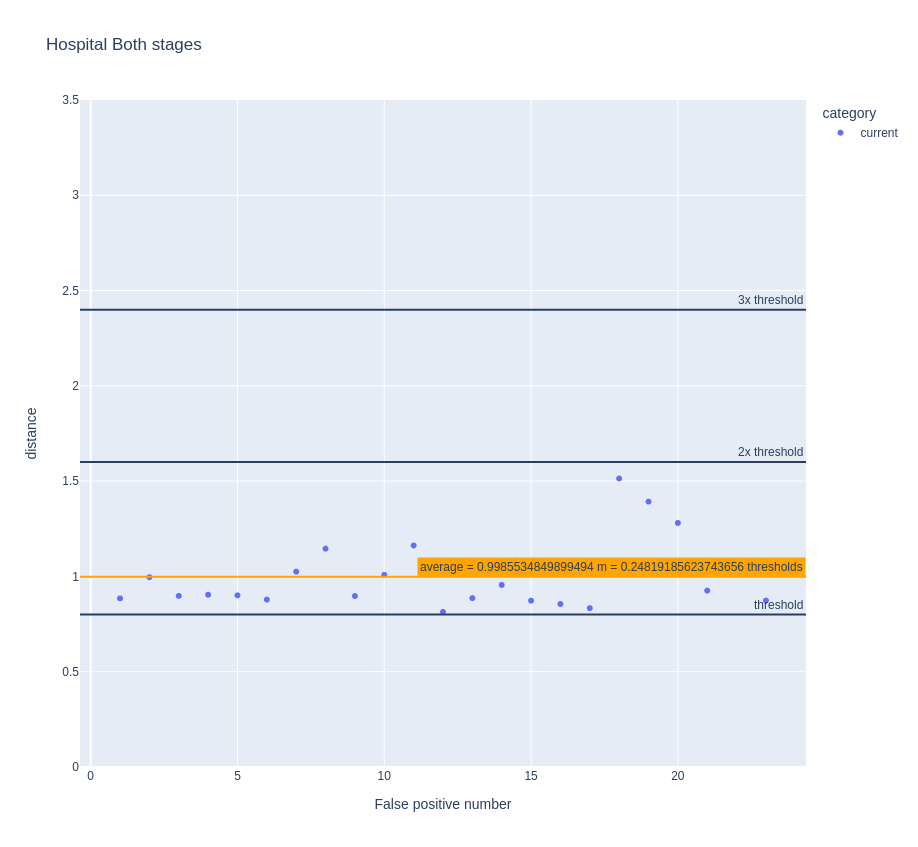
\includegraphics[width=0.5\textwidth]{hospitalBothStagesFalsePositiveDistances.png}\label{fig:FPErr32}}
    \caption{False positive distances in the hospital environment}
    \label{fig:averageFPErrorHospital}
\end{figure}

\begin{table}[htpb]
    \caption{Average and maximal errors of false positive evaluations in different environments}\label{tab:averageFPError}
    \centering
    \begin{tabular}{l | l  l| l l| l l}
        \toprule
        \textbf{}          & \multicolumn{2}{l|}{\textbf{1st stage only}} & \multicolumn{2}{l|}{\textbf{both stages}} & \multicolumn{2}{l}{\textbf{OpenRatSLAM}}                             \\
        {}                 & avg                                          & max                                       & avg                                      & max    & avg    & max     \\
        \hline
        \textbf{Warehouse} & 1.32 m                                       & 3.06 m                                    & 1.39 m                                   & 3.06 m & 8.93 m & 11.52 m \\
        \textbf{House}     & 0.93 m                                       & 1.16 m                                    & 0.99 m                                   & 1.39 m & 1.84 m & 3.93 m  \\
        \textbf{Hospital}  & 1.00 m                                       & 1.52 m                                    & 1.00 m                                   & 1.51 m & 6.56 m & 14.57 m \\
        \bottomrule
    \end{tabular}
\end{table}

As the results show, both techniques suggested in this work showed outstanding performance in this metric. In the house and hospital environment, the average error lies only 13-20 cm away from the threshold, which is less than 25 \% of the threshold size. Moreover, all evaluated false negatives in these environments are not farther than twice the threshold from the matched scene. This means that all wrongly evaluated matches are still very close to the threshold and shouldn't cause almost any damage to the final result. Some errors in the warehouse environment were slightly larger, but they were only exceptional cases, and most of the wrongly classified matches are still very close to the threshold.\par
On the other hand, the results of the visual place recognition used in the OpenRatSLAM were significantly worse. As the results suggest, most of the wrongly evaluated scenes were spread over the whole environment, and the distances between the incorrectly matched scenes were huge. The most significant errors can be observed in the hospital environment, which drastically influenced the generated experience map, as discussed in the section \ref{section:RatSalmIntegration}.\par
According to this metric, both presented approaches significantly outperformed the visual place recognition used in the original RatSLAM.
